
% vim:set ff=unix expandtab ts=2 sw=2:


%\the\textheight
	\setlength{\TPHorizModule}{1\textwidth} % our coordinates are <1
	\setlength{\TPVertModule}{\TPHorizModule}
	\textblockorigin{50mm}{200mm}
	%start everything near the top-left corner
	\setlength{\parindent}{0pt} % 
	\definecolor{myblue}{RGB}{128,128,255}
	\definecolor{myred}{RGB}{255,128,128}

	\begin{textblock}{0.2}(0,0)
		This Block ck 3 modules wide, and is placed with its top left corner
		 ‘origin’ on the page. Note that the length of the block is not
		specified in the arguments -- the box will be as long as necessary to
		accomodate the text inside it.
		You need to examine the output of the
		text to adjust the positioning of the blocks on the page.
	\end{textblock}
	\begin{textblock}{.2}(.1,.2)
	  \textblocklabel{block two} 
    \begin{block}{Beamer Block inside}
      \begin{minipage}[t][50cm][t]{\textwidth}	
		    Here is another, slightly narrower, block, at position (.1,.2) on the page.
        That contains a beamer block environment, which contains a minipage to 
        have some (indirect) control over the size of the box.
        % vim:set ff=unix expandtab ts=2 sw=2:
        \alert{\textit{Example with pictures:}}
        \begin{itemize}
        	\item we add a pseudo picture
        \end{itemize}
        \vspace{1cm}
        \begin{columns}
        \column{.8\textwidth}
        	\begin{figure}[tb]
        	\begin{center}
        		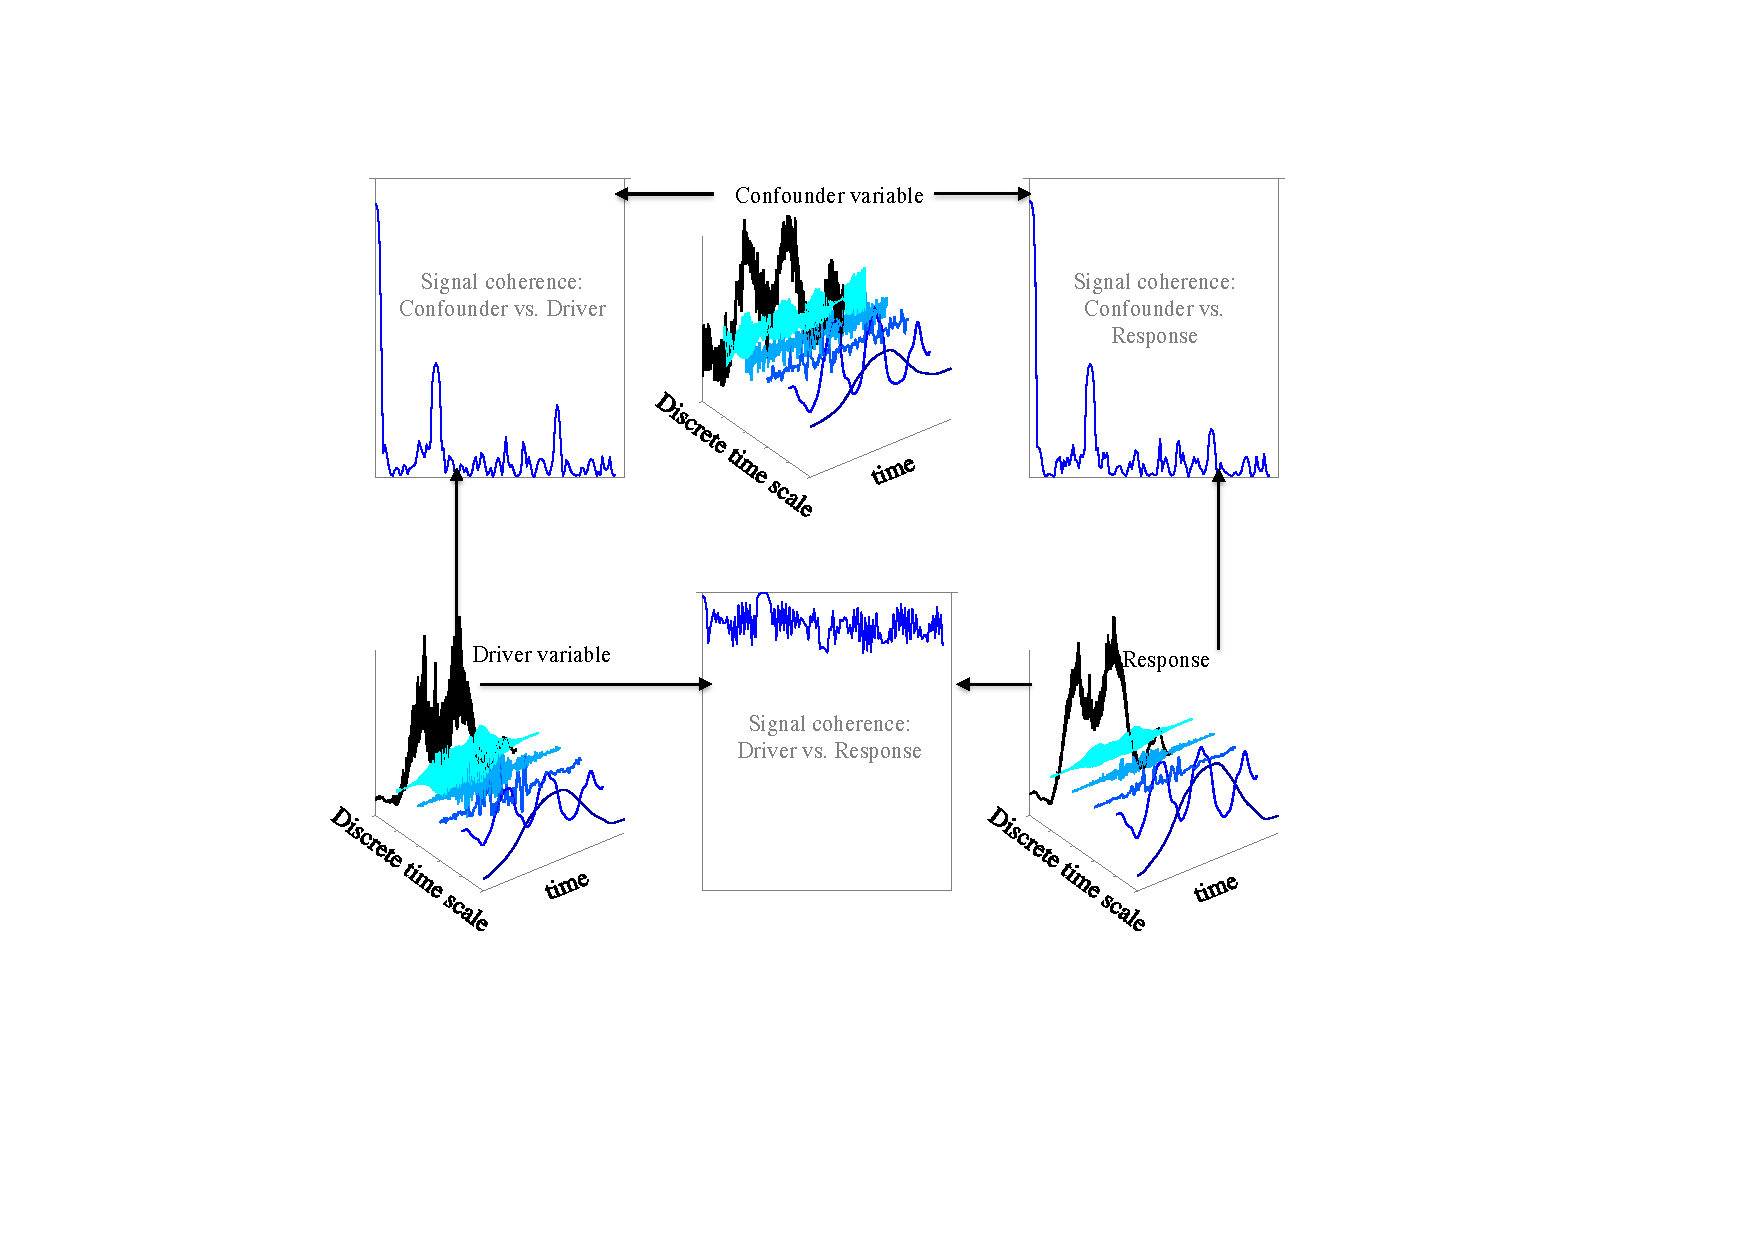
\includegraphics[width=.55\textwidth]{images/content/FIG1.pdf}
        	\end{center}
        	\end{figure}
        \column{.2\textwidth}
        \small{\textit{a pseudo caption}}
        \vspace{4cm}
        	\begin{figure}[tb]
        		
\includegraphics[width=.6\textwidth]{images/qrcode-RSCAPE.jpg}
        	\end{figure}
        \end{columns}
        \vspace{1cm}
        We add some text here to show that the block will grow even over the bottom of the column. This demonstrates
      \end{minipage}
    \end{block}
   \end{textblock}

   \textblockcolor{myblue}
   \begin{textblock}{.3}(.2,.8)
     The textblocks can also overlap.
     To make the effect more visible we also used 
     \begin{verbatim}
       \textblockcolor{myblue}
     \end{verbatim}
	 \end{textblock}
   
   \textblockcolor{white}
   \begin{textblock}{.3}[0.5,0.5](.2,.9)
		This is at position (2,3), but because the optional argument
		[0.5,0.5]
		has been given, it is the centre of the block which is
		located at that point, rather than the top-left corner.
	\end{textblock}
  % lets build our own environment with 
  % a minibox inside to be able to influence
  % the vertical 
  \newenvironment{mybox}[3]{
	  \begin{textblock*}{#1}#2
  	  \begin{minipage}[t][#3][t]{\textwidth}	
  }
  {
	    \end{minipage}
	  \end{textblock*}
  }
  %% now we set some lengths to organize our boxes in columns 
  %% for both columns
  \newlength{\vblocksep}
  \setlength{\vblocksep}{1cm} 
  \newlength{\hblocksep}
  \setlength{\hblocksep}{1cm} 
  \newlength{\xcols}
  \setlength{\xcols}{0.4\textwidth} 
  \newlength{\hcols}
  \setlength{\hcols}{80cm} %overall height of columns (fixme: this should ideally be set in the template)
  \newlength{\wcols}
  \setlength{\wcols}{40cm} %overall width of our columns
  %% column specific
  %% colA
  \newlength{\wcolA}
  % set the widht of the first column manually
  \setlength{\wcolA}{.41\wcols} 
  \newlength{\hboxOneA} 
  % set the height of the first box manually
  \setlength{\hboxOneA}{15cm}
  \newlength{\hboxTwoA}
  % compute the height of the second box 
  \setlength{\hboxTwoA}{ \dimexpr ( \hcols - \hboxOneA) \relax}
  
  %% now draw the actual boxes
  % columnA
  \begin{mybox}{\wcolA}{(\xcols,0cm)}{\hboxOneA}
      
% vim:set ff=unix expandtab ts=2 sw=2:
Since our poster template uses the beamer class,
we can influence the defaults for beamer blocks by the template.
(for example the background and foreground colors, fonts and fontsize for content and header of this box)
Which can help to avoid a lot of formatting in the user code andmakes it easier to achieve a standard layout.
The interior is quite flexible.\\
\begin{itemize}
	\item we add a pseudo picture
\end{itemize}
	\begin{figure}[tb]
		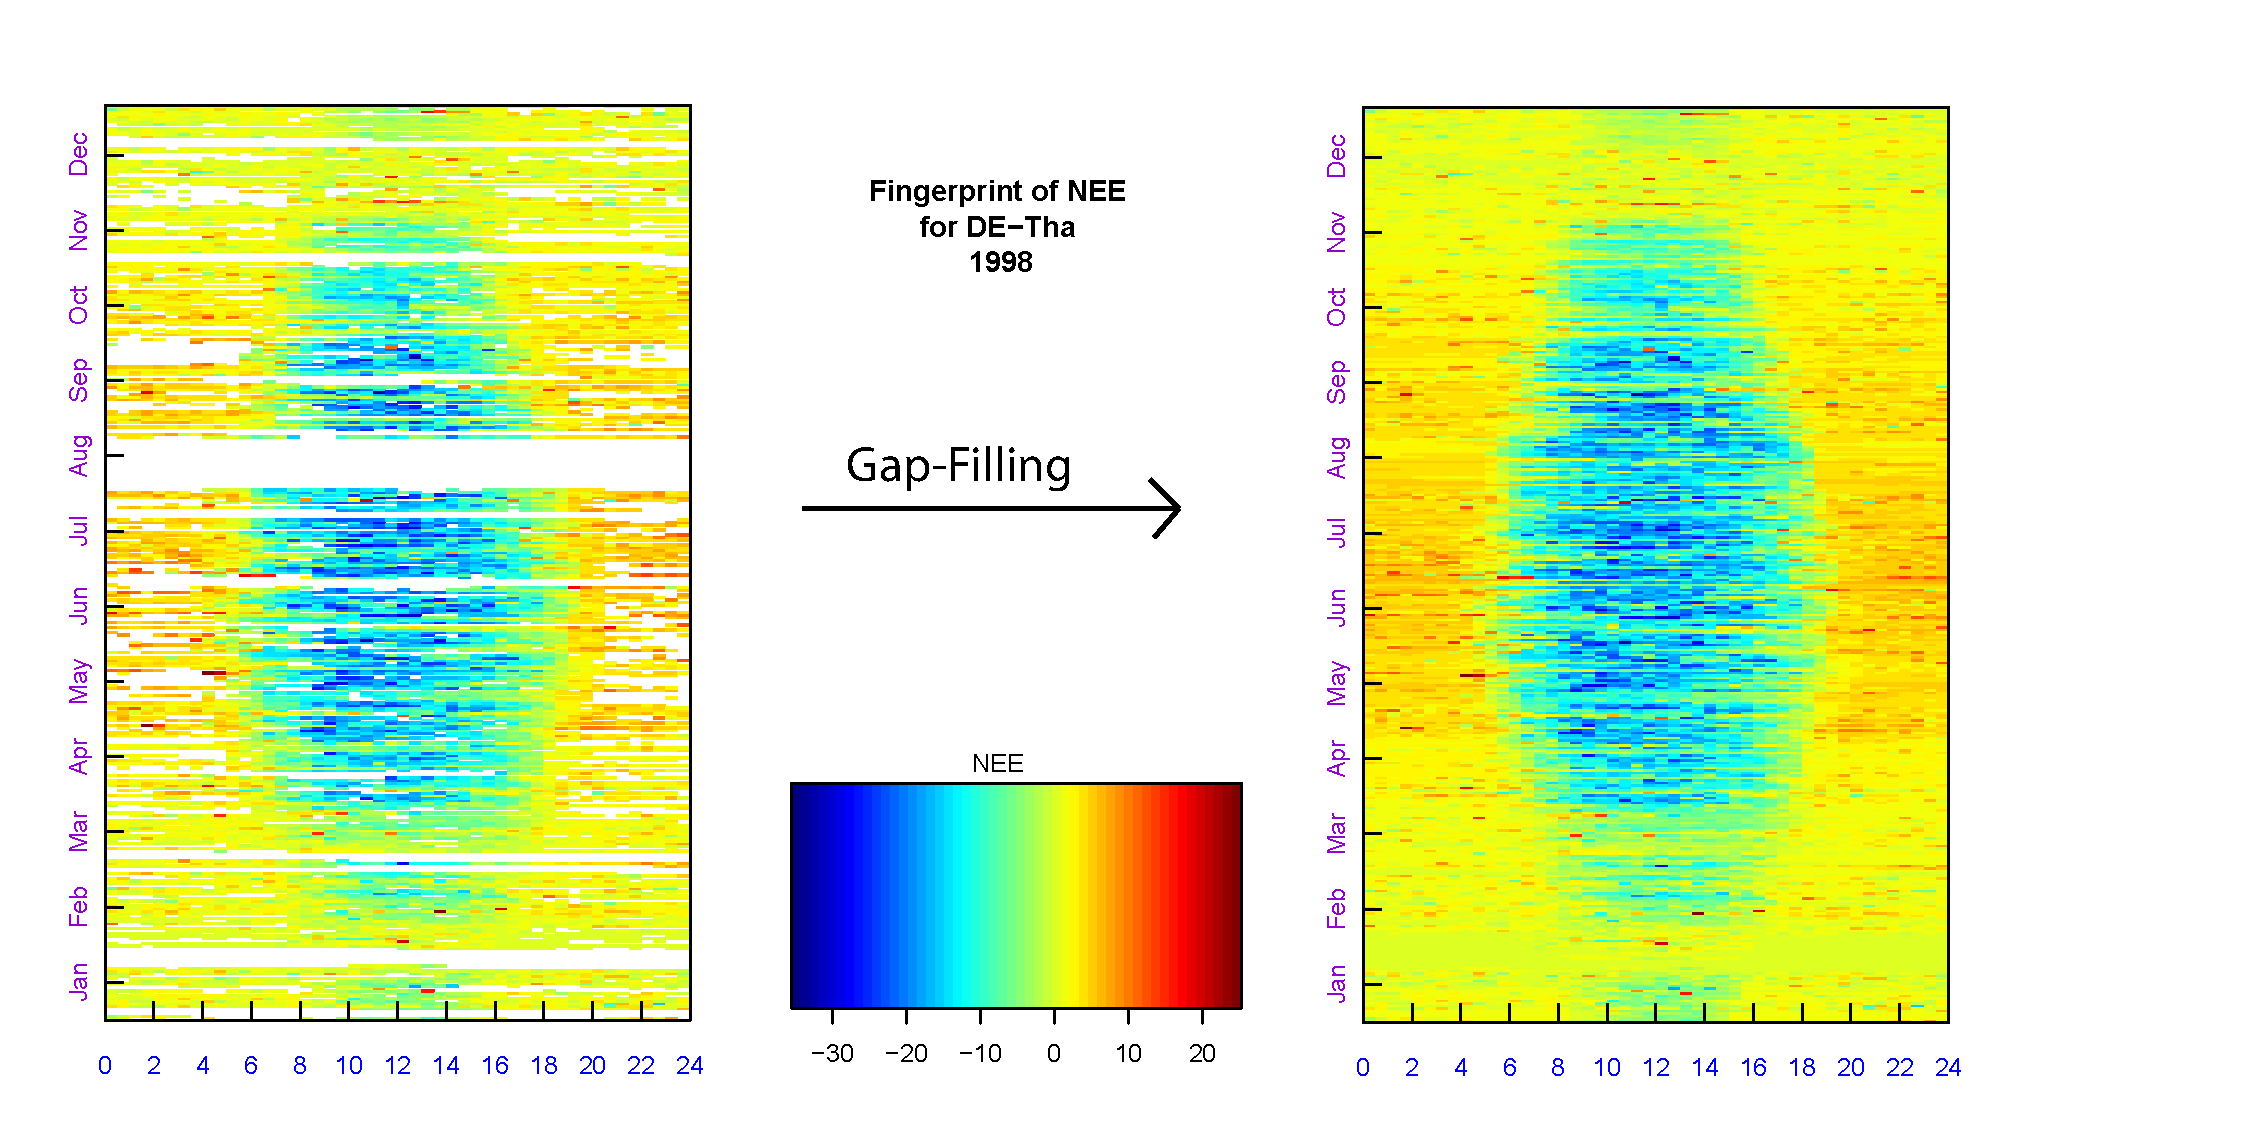
\includegraphics[height=3cm]{images/content/DE-Tha_1998_FP_NEE_ffc.pdf}
    \caption{a pseudo caption}
	\end{figure}




  \end{mybox}
  \begin{mybox}{\wcolA}{(\xcols,\dimexpr \hboxOneA + \vblocksep \relax )}{\hboxTwoA}
    
% vim:set ff=unix expandtab ts=2 sw=2:
Beamer boxes can be used inside the columns environment, also provided by the beamer class.
This simplifies some common vertical and horizontal alignment tasks.
\alert{However there is one notable exception that requires a hack:}\\

It is not possible to directly align beamer blocks vertically 
at the top \alert{AND} the bottom of the poster simultaneously for the following reason.
The block environment has no \emph{height} parameter. 
The blocks grow with their content and the header.
We can influence there size only indirectly by wrapping their content in minipages.
The following code defines a minimal environment that allows 
to add extra white space to the blocks.
\inputminted{latex}{content/myBox.tex}
With control over the vertical extent established, we can choose the size of the first box in a column and then use
\LaTeX2e s built in computing facilities (
  \verb1 \dimexpr1 and \verb1 \numexpr1) to determine the size of the second box.
\inputminted{LaTeX}{content/lengths.tex}



  \end{mybox}

  
  %% column specific
  %% colB
  \newlength{\wcolB}
  % compute the width of the second column 
  \setlength{\wcolB}{\dimexpr \wcols-\wcolA \relax} 
  \newlength{\hboxOneB}
  % columnB
  % Ttis time we even go a step further and measure
  % the contents of the first box before we draw it
  %\newsavebox\myMeasuringBox
  \setbox0=\vtop{%
  	\begin{minipage}[t]{\wcolB}	
      
% vim:set ff=unix expandtab ts=2 sw=2:
  {\vspace{.2cm}\textbf{REddyProc}\hfill\normalsize{her could be some names}}
\alert{\textit{Context:}}

To measure how much space this box will take we put it in a 
savebox:


	  \end{minipage}
  }
  \setlength{\hboxOneB}{\ht0}%
  \addtolength{\hboxOneB}{\dp0}%
  \newlength{\hboxTwoB}
  % compute the height of the second box 
  \setlength{\hboxTwoB}{ \dimexpr ( \hcols - \hboxOneB) \relax}
  
  \newlength{\xcolB}
  \setlength{\xcolB}{\dimexpr \xcols+\wcolA+\hblocksep \relax } 
  \begin{mybox}{\wcolB}{(\xcolB,0cm)}{\hboxOneB}
   \usebox0  
  \end{mybox}
  \begin{mybox}{\wcolB}{(\xcolB,\dimexpr \hboxOneB + \vblocksep \relax )}{\hboxTwoB}
    
% vim:set ff=unix expandtab ts=2 sw=2:
Beamer boxes can be used inside the columns environment, also provided by the beamer class.
This simplifies some common vertical and horizontal alignment tasks.
\alert{However there is one notable exception that requires a hack:}\\

It is not possible to directly align beamer blocks vertically 
at the top \alert{AND} the bottom of the poster simultaneously for the following reason.
The block environment has no \emph{height} parameter. 
The blocks grow with their content and the header.
We can influence there size only indirectly by wrapping their content in minipages.
The following code defines a minimal environment that allows 
to add extra white space to the blocks.
\inputminted{latex}{content/myBox.tex}
With control over the vertical extent established, we can choose the size of the first box in a column and then use
\LaTeX2e s built in computing facilities (
  \verb1 \dimexpr1 and \verb1 \numexpr1) to determine the size of the second box.
\inputminted{LaTeX}{content/lengths.tex}



  \end{mybox}
